\documentclass{beamer}
\usepackage{hyperref}
\usepackage[T1]{fontenc}


% other packages
\usepackage{latexsym,amsmath,xcolor,multicol,booktabs}
\usepackage{graphicx,pstricks,listings,stackengine}
\usepackage{tikz}
\usetikzlibrary{shapes.geometric, arrows.meta, positioning, calc, decorations.pathreplacing}
\usepackage{pgfplots}
\pgfplotsset{compat=1.18}

% Custom Colors from your TiKZ file
\definecolor{myBlue}{RGB}{70, 130, 180}
\definecolor{myOrange}{RGB}{255, 140, 0}
\definecolor{myGreen}{RGB}{60, 179, 113}

% --- UPDATE YOUR DETAILS HERE ---
\author{Cedric Damais, Yacine Benihaddadene, Amine Mike El Maalouf, Leon Ayral, Oscar Le Dauphin} % Change this to your name
\title{IWAE vs. VAE}
\subtitle{Tighter Bounds, Richer Latents?}
\institute{GAIDM \\ EPITA}
\date{\today} 

% Load the custom theme
\usepackage{NJUPT}

% defs (Kept from your template)
\def\cmd#1{\texttt{\color{red}\footnotesize $\backslash$#1}}
\def\env#1{\texttt{\color{blue}\footnotesize #1}}
\definecolor{deepblue}{rgb}{0,0,0.5}
\definecolor{deepred}{rgb}{0.6,0,0}
\definecolor{deepgreen}{rgb}{0,0.5,0}
\definecolor{halfgray}{gray}{0.55}

\lstset{
    basicstyle=\ttfamily\small,
    keywordstyle=\bfseries\color{deepblue},
    emphstyle=\ttfamily\color{deepred},
    stringstyle=\color{deepgreen},
    numbers=left,
    numberstyle=\small\color{halfgray},
    rulesepcolor=\color{red!20!green!20!blue!20},
    frame=shadowbox,
}

\begin{document}

% Title Page
\begin{frame}
    \titlepage
    \begin{figure}[htpb]
        \begin{center}
            % Keep the Logo if you want it
            \includegraphics[width=0.2\linewidth]{pic/epita-logo.png}
        \end{center}
    \end{figure}
\end{frame}

% Table of Contents
\begin{frame}
    \tableofcontents[sectionstyle=show,subsectionstyle=show/shaded/hide,subsubsectionstyle=show/shaded/hide]
\end{frame}

% =======================================================
% SECTION 1: THEORY
% =======================================================
\section{Introduction \& Theory}

\begin{frame}{The Goal: Latent Variable Inference}
    \textbf{The Objective:} Given data $x$, we want to learn the posterior distribution of the latent variables $z$:
    
    $$ p(z|x) = \frac{p(x|z)p(z)}{p(x)} $$
    
    \begin{itemize}
        \item $p(x|z)$: Likelihood (Decoder)
        \item $p(z)$: Prior (e.g., $\mathcal{N}(0,I)$)
        \item \textbf{$p(x)$: Marginal Likelihood (The Evidence)}
    \end{itemize}

    \vspace{1em}
    
    \begin{alertblock}{The Problem: Intractability}
        We can't simply use Bayes Formula because p(x) is intractable. To calculate the denominator $p(x)$, we must marginalize out $z$:
        $$ p(x) = \int p(x|z)p(z) \, dz $$
        \begin{itemize}
            \item This integral is \textbf{intractable} for complex neural networks.
            \item \textbf{Consequence:} We cannot compute $p(z|x)$ analytically.
            \item \textbf{Solution:} Approximate $p(z|x)$ with $q_\phi(z|x)$ (Variational Inference).
        \end{itemize}
    \end{alertblock}
\end{frame}

\begin{frame}{Standard VAE: The Objective}
    \textbf{Goal:} Maximize marginal log-likelihood $\log p(x)$.
    \vspace{0.5em}
    
    Since $p(x)$ is intractable, VAE ($K=1$) maximizes the \textbf{ELBO}:
    $$ \log p(x) \ge \mathcal{L}_{\text{VAE}} = \mathbb{E}_{z \sim q} \left[ \log \frac{p(x,z)}{q(z|x)} \right] $$

    \vspace{1em}
    
    \begin{alertblock}{The Problem: The "Gap"}
        The bound is strictly lower than the evidence due to the KL divergence:
        $$ \log p(x) - \mathcal{L}_{\text{VAE}} = \text{KL}(q(z|x) || p(z|x)) $$
    \end{alertblock}
    
    \begin{itemize}
        \item If $q(z|x)$ is too simple $\rightarrow$ \textbf{Loose Bound}.
        \item Loose bound $\rightarrow$ Risk of \textbf{Posterior Collapse}.
    \end{itemize}
\end{frame}

\begin{frame}{Model Architecture}
    \centering
    % Resizebox ensures the graph fits the slide width automatically
    \resizebox{0.95\textwidth}{!}{%
        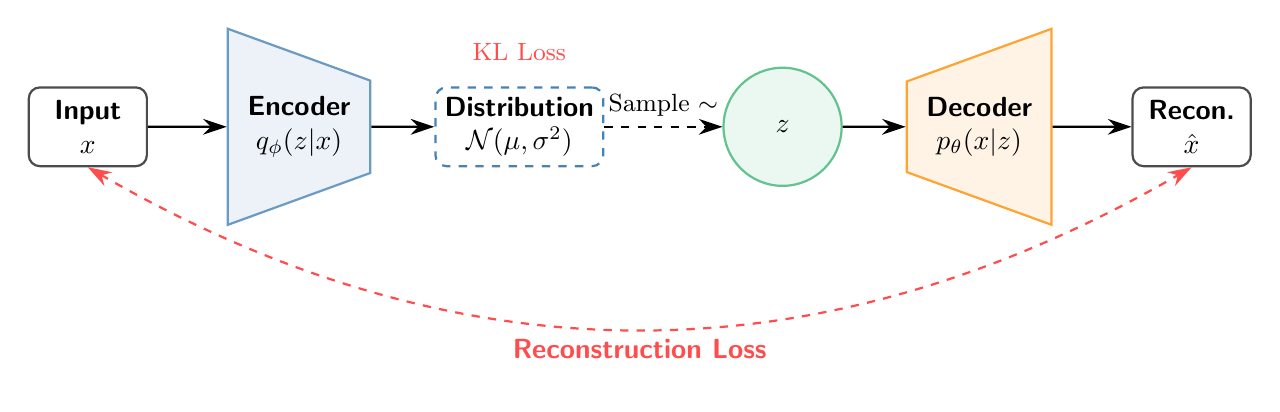
\begin{tikzpicture}[
            node distance=1.5cm,
            font=\sffamily\bfseries,
            >={Stealth[length=3mm, width=2mm]},
            % Styles
            box/.style={
                draw=black!70, thick, align=center, minimum height=1cm, minimum width=1.5cm, fill=white, rounded corners
            },
            trapezium_enc/.style={
                trapezium, trapezium angle=70, draw=myBlue!80, thick, fill=myBlue!10, 
                align=center, minimum height=1.5cm, minimum width=2.5cm, shape border rotate=270
            },
            trapezium_dec/.style={
                trapezium, trapezium angle=70, draw=myOrange!80, thick, fill=myOrange!10, 
                align=center, minimum height=1.5cm, minimum width=2.5cm, shape border rotate=90
            },
            latent/.style={
                circle, draw=myGreen!80, thick, fill=myGreen!10, align=center, minimum size=1.5cm
            }
        ]

            % --- Nodes ---

            % 1. Input
            \node[box] (x) {Input\\$x$};

            % 2. Encoder (Compressing)
            \node[trapezium_enc, right=1cm of x] (encoder) {Encoder\\$q_\phi(z|x)$};

            % 3. Distribution Parameters (Merged mu/sigma)
            \node[box, right=0.8cm of encoder, draw=myBlue, dashed] (dist) {Distribution\\$\mathcal{N}(\mu, \sigma^2)$};

            % 4. Latent Variable (Sampling)
            \node[latent, right=1.5cm of dist] (z) {$z$};

            % 5. Decoder (Expanding)
            \node[trapezium_dec, right=0.8cm of z] (decoder) {Decoder\\$p_\theta(x|z)$};

            % 6. Output
            \node[box, right=1cm of decoder] (xhat) {Recon.\\$\hat{x}$};

            % --- Arrows ---
            \draw[->, thick] (x) -- (encoder);
            \draw[->, thick] (encoder) -- (dist);
            
            % Sampling Arrow
            \draw[->, thick, dashed] (dist) -- node[midway, above, font=\small\normalfont, text=black] {Sample $\sim$} (z);
            
            \draw[->, thick] (z) -- (decoder);
            \draw[->, thick] (decoder) -- (xhat);

            % --- Loss Annotation ---
            \draw[<->, red!70, dashed, thick] (x.south) to[bend right=30] node[midway, below] {Reconstruction Loss} (xhat.south);
            
            \node[above=0.2cm of dist, text=red!70, font=\small] {KL Loss};

        \end{tikzpicture}%
    }
\end{frame}

\section{The IWAE Solution}

\begin{frame}{Novelty 1: Strictly Tighter Bounds}
    \textbf{Theorem (Burda et al., 2015):}
    The IWAE bound $\mathcal{L}_K$ is monotonically increasing with $K$.
    
    $$ \mathcal{L}_1 \le \mathcal{L}_2 \le \dots \le \mathcal{L}_K \le \dots \le \log p(x) $$

    \vspace{0.5em}

    \begin{block}{Why?}
        Using \textbf{Jensen's Inequality} on the concave log function:
        $$ \mathbb{E} \left[ \log \left( \frac{1}{K} \sum w_i \right) \right] \le \log \left( \mathbb{E} \left[ \frac{1}{K} \sum w_i \right] \right) = \log p(x)$$
    \end{block}

    \textbf{Implication:}
    \begin{itemize}
        \item As $K \to \infty$, the estimator converges to the true marginal likelihood $\log p(x)$.
        \item Even with a finite $K$, we are guaranteed a better objective than VAE.
    \end{itemize}
\end{frame}

\begin{frame}{Novelty 2: Richer Implicit Posteriors}
    \centering
    \textbf{The IWAE Solution: Weighting as Filtering}
    
    \vspace{1em}

    % 1. The Normalization (The Filter)
    $$ \text{Normalized Weight: } \quad \tilde{w}_i = \frac{w_i}{\sum_{j=1}^k w_j} \quad \text{where} \quad w_i = \frac{p(x,z_i)}{q(z_i|x)} $$

    \vspace{1em}

    % 2. The Implicit Posterior (The Result)
    $$ \underbrace{\tilde{q}(z|x)}_{\substack{\text{Implicit} \\ \text{Multi-modal}}} \approx \sum_{i=1}^k \tilde{w}_i \delta(z - z_i) $$

    \vspace{1em}

    % 3. The Gradient Update (The Mechanism)
    $$ \nabla \mathcal{L}_k = \mathbb{E}_{\epsilon} \left[ \sum_{i=1}^{k} \textcolor{red}{\tilde{w}_i} \nabla_\theta \log w(x, z_i, \theta) \right] $$
    
    \vspace{0.5em}
    
    \begin{center}
        \textcolor{red}{\textbf{$\uparrow$ High $\tilde{w}_i$ dominates the gradient update}}
    \end{center}

\end{frame}

\begin{frame}{Why Sampling More Helps? (The Mechanics)}
    
    \begin{columns}[T]
        % --- LEFT: The Problem ---
        \begin{column}{0.48\textwidth}
            \begin{alertblock}{Case $K=1$ (Risky)}
                If we draw just \textbf{one} bad sample $z_1$:
                $$ w_1 \approx 0 $$
                $$ \log(w_1) \to \textcolor{red}{-\infty} $$
                \vspace{0.5em}
                \centering
                \textbf{{Gradient Explodes}}
            \end{alertblock}
        \end{column}

        % --- RIGHT: The Solution ---
        \begin{column}{0.48\textwidth}
            \begin{exampleblock}{Case $K > 1$ (Hedging)}
                If we draw many bad samples, but just \textbf{one good one}:
                $$ \log(0 + 0 + \dots + \textcolor{blue}{\mathbf{w_{good}}}) $$
                $$ \approx \log(\textcolor{blue}{\mathbf{w_{good}}}) > -\infty $$
                \vspace{0.5em}
                \centering
                \textbf{Stable Training}
            \end{exampleblock}
        \end{column}
    \end{columns}

    \vspace{2em}

    % Bottom Takeaway
    \centering
    \textbf{The Insight:} The sum acts as a safety net. The Encoder is allowed to make mistakes, as long as it gets it right \textit{once}.

\end{frame}

\begin{frame}{The Mechanism: Importance Weighting}
    \vspace{0.5em}
    \begin{columns}[T] % T aligns columns at the top
        % --- LEFT: The Math ---
        \begin{column}{0.48\textwidth}
            \textbf{1. The Definition}
            \begin{itemize}
                \item Calculate raw weight:
                $$ w_i = \frac{p(x,z_i)}{q(z_i|x)} $$
                \item Normalize:
                $$ \tilde{w}_i = \frac{w_i}{\sum_{j=1}^k w_j} $$
            \end{itemize}
        \end{column}

        % --- RIGHT: The Intuition ---
        \begin{column}{0.48\textwidth}
            \textbf{2. The Intuition}
            \vspace{1em}
            \begin{itemize}
                \item[] Sample $z_i$ is \textbf{Good}
                \par $\to p(x,z_i)$ is High
                \par $\to \textcolor{green}{\mathbf{\tilde{w}_i \approx 1}}$
                \vspace{1em}
                \item[] Sample $z_j$ is \textbf{Bad}
                \par $\to p(x,z_j)$ is Low
                \par $\to \textcolor{red}{\mathbf{\tilde{w}_j \approx 0}}$
            \end{itemize}
        \end{column}
    \end{columns}

    \vspace{1.5em}

    % --- BOTTOM: The Takeaway ---
    \begin{block}{Key Result: The Filter Effect}
        The gradient update effectively \textbf{ignores} bad samples:
        $$ \nabla \theta \approx \sum_{i=1}^{k} \underbrace{\textcolor{blue}{\mathbf{\tilde{w}_i}}}_{\text{Quality Score}} \cdot \nabla \log w(x, z_i) $$
    \end{block}
\end{frame}

\begin{frame}{IWAE Architecture}
    \centering
    \resizebox{1.0\textwidth}{!}{%
    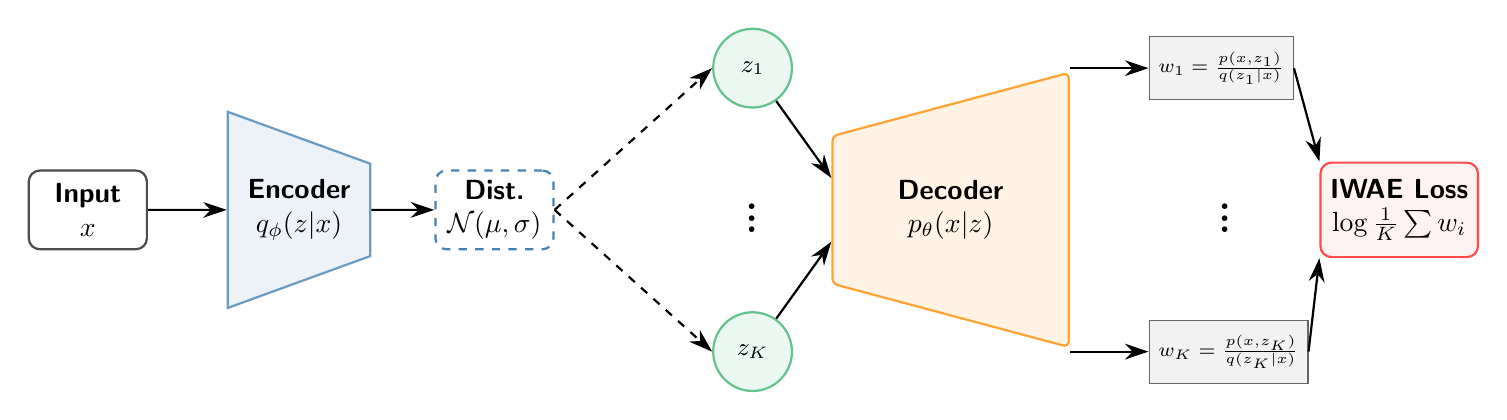
\begin{tikzpicture}[
    node distance=1.5cm,
    font=\sffamily\bfseries,
    >={Stealth[length=3mm, width=2mm]},
    % Styles
    box/.style={
        draw=black!70, thick, align=center, minimum height=1cm, minimum width=1.5cm, fill=white, rounded corners
    },
    trapezium_enc/.style={
        trapezium, trapezium angle=70, draw=myBlue!80, thick, fill=myBlue!10, 
        align=center, minimum height=1.5cm, minimum width=2.5cm, shape border rotate=270
    },
    % LARGE TRAPEZOID DECODER
    large_decoder/.style={
        trapezium, trapezium angle=75, draw=myOrange!80, thick, fill=myOrange!10, 
        align=center, minimum height=3.0cm, minimum width=1.0cm, shape border rotate=90, rounded corners=2pt
    },
    latent/.style={
        circle, draw=myGreen!80, thick, fill=myGreen!10, align=center, minimum size=1.0cm, font=\small
    },
    weight/.style={
        draw=black!60, thin, fill=gray!10, minimum height=0.8cm, minimum width=1.3cm, font=\scriptsize, align=center
    },
    loss_box/.style={
        draw=red!70, thick, fill=red!5, align=center, minimum height=1.2cm, minimum width=2cm, rounded corners
    }
]

    % --- 1. Input & Encoder ---
    \node[box] (x) {Input\\$x$};
    \node[trapezium_enc, right=1cm of x] (encoder) {Encoder\\$q_\phi(z|x)$};
    \node[box, right=0.8cm of encoder, draw=myBlue, dashed] (dist) {Dist.\\$\mathcal{N}(\mu, \sigma)$};

    % --- 2. The K Samples ---
    % Positioned vertically
    \node[latent, right=2cm of dist, yshift=1.8cm] (z1) {$z_1$};
    \node[latent, right=2cm of dist, yshift=-1.8cm] (zk) {$z_K$};
    
    % Sampling Arrows
    \draw[->, thick, dashed] (dist.east) -- (z1.west);
    \draw[->, thick, dashed] (dist.east) -- (zk.west);
    
    % Vertical dots
    \path (z1) -- (zk) node[midway, font=\Huge] {$\vdots$};

    % --- 3. The Single Decoder (Trapezoid) ---
    % --- 3. The Single Decoder (Trapezoid) ---
    % 'minimum height' controls the vertical size (5.5cm)
    % 'minimum width' controls the horizontal size (3.5cm)
    \node[large_decoder, right=1.0cm of $(z1)!0.5!(zk)$, minimum height=3.0cm, minimum width=2.0cm] (decoder) {Decoder\\$p_\theta(x|z)$};
    
    % --- Connecting Z arrows to the BACK (Left Side) ---
    % We use angle anchors to force the connection to the Left side.
    % 180 is left. 165 is slightly up-left. 195 is slightly down-left.
    
    \draw[->, thick] (z1) -- (decoder.165);
    \draw[->, thick] (zk) -- (decoder.195);
    % --- 4. Importance Weights (Outputs) ---
    \node[weight, right=1.0cm of decoder, yshift=1.8cm] (w1) {$w_1 = \frac{p(x,z_1)}{q(z_1|x)}$};
    \node[weight, right=1.0cm of decoder, yshift=-1.8cm] (wk) {$w_K = \frac{p(x,z_K)}{q(z_K|x)}$};
    
    % Dots between weights
    \path (w1) -- (wk) node[midway, font=\Huge] {$\vdots$};

    % Arrows exiting decoder
    % We anchor them to the right side of the trapezoid
    \draw[->, thick] (decoder.east |- w1) -- (w1);
    \draw[->, thick] (decoder.east |- wk) -- (wk);

    % --- 5. Aggregation & Loss ---
    \node[loss_box, right=1.2cm of $(w1)!0.5!(wk)$] (loss) {\textbf{IWAE Loss}\\$\log \frac{1}{K} \sum w_i$};

    % Connect weights to loss
    \draw[->, thick] (w1.east) -- (loss.north west);
    \draw[->, thick] (wk.east) -- (loss.south west);

    % --- Standard Connections ---
    \draw[->, thick] (x) -- (encoder);
    \draw[->, thick] (encoder) -- (dist);


\end{tikzpicture}
    }
\end{frame}

% =======================================================
% SECTION 2: METHODOLOGY
% =======================================================
\section{Methodology}

\begin{frame}{Experimental Setup}
    \begin{itemize}
        \item \textbf{Objective:} Compare VAE ($K=1$) vs IWAE ($K>1$).
        \item \textbf{Constraint:} \textbf{Identical Architecture} for fair comparison.
    \end{itemize}

    \vspace{0.5em}

    \begin{table}[h]
        \centering
        \begin{tabular}{c|c}
            \toprule
            \textbf{Parameter} & \textbf{Value} \\
            \midrule
            Dataset & MNIST (Binarized) \\
            Encoder & MLP ($784 \to 400 \to 20$) \\
            Decoder & MLP ($20 \to 400 \to 784$) \\
            Optimizer & Adam ($lr=1e-3$) \\
            \textbf{K (Samples)} & \textbf{1, 5, 20, 30, 50, 100} \\
            \bottomrule
        \end{tabular}
    \end{table}

    \begin{exampleblock}{Implementation Detail}
        Used \texttt{torch.logsumexp} to avoid numerical underflow.
    \end{exampleblock}
\end{frame}

% =======================================================
% SECTION 3: RESULTS
% =======================================================
\section{Results}

\subsection{Log-Likelihood}
\begin{frame}{Result 1: Estimated Log-Likelihood vs Number of Samples (K)}
    \begin{itemize}
        \item \textbf{Metric:} Estimated Log-Likelihood (Higher is better).
    \end{itemize}

    \begin{figure}[htpb]
        \centering
        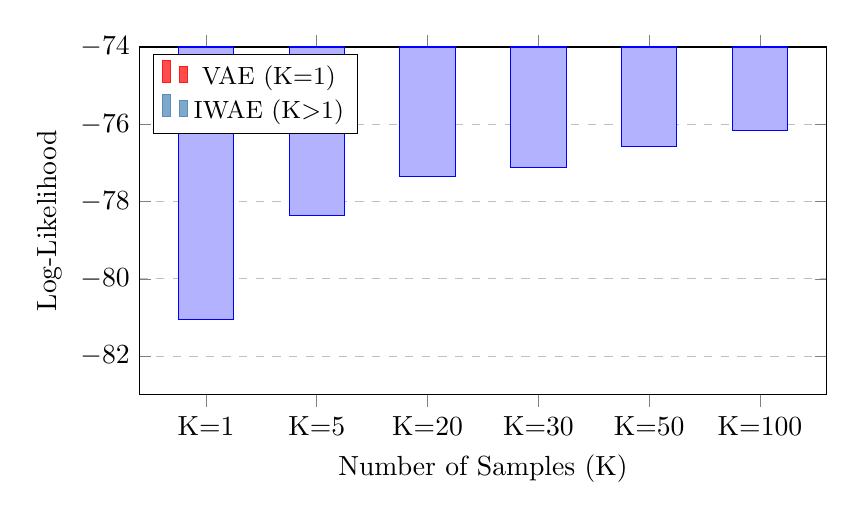
\begin{tikzpicture}
            \begin{axis}[
                ybar,
                width=0.85\textwidth,
                height=6cm,
                ylabel={Log-Likelihood},
                xlabel={Number of Samples (K)},
                symbolic x coords={K=1, K=5, K=20, K=30, K=50, K=100},
                xtick=data,
                ymin=-83,
                ymax=-74,
                nodes near coords,
                nodes near coords align={vertical},
                every node near coord/.append style={font=\scriptsize},
                bar width=20pt,
                enlarge x limits=0.12,
                legend style={at={(0.02,0.98)}, anchor=north west, font=\small},
                ymajorgrids=true,
                grid style=dashed,
                scatter,
                scatter src=explicit symbolic,
                scatter/classes={
                    vae={fill=red!70, draw=red!90},
                    iwae={fill=myBlue!70, draw=myBlue!90}
                },
            ]
            \addplot coordinates {
                (K=1, -81.06) [vae]
                (K=5, -78.36) [iwae]
                (K=20, -77.34) [iwae]
                (K=30, -77.12) [iwae]
                (K=50, -76.58) [iwae]
                (K=100, -76.17) [iwae]
            };
            \addlegendimage{fill=red!70, draw=red!90, area legend}
            \addlegendentry{VAE (K=1)}
            \addlegendimage{fill=myBlue!70, draw=myBlue!90, area legend}
            \addlegendentry{IWAE (K$>$1)}
            \end{axis}
        \end{tikzpicture}
        \caption{Estimated Log-Likelihood on MNIST Test Set (Higher is Better)}
    \end{figure}

    \textbf{Observation:} $\mathcal{L}_{100} > \mathcal{L}_{50} > \mathcal{L}_{20} > \mathcal{L}_{5} > \mathcal{L}_{1}$. Increasing $K$ strictly tightens the bound.
\end{frame}

\subsection{Latent Utilization}
\begin{frame}{Result 2: Active Latent Units vs Number of Samples (K)}
    \begin{itemize}
        \item \textbf{Metric:} Active Units (Dimensions where $\text{KL} > \epsilon$, with $\epsilon = 0.01$).
    \end{itemize}

    \begin{figure}[htpb]
        \centering
        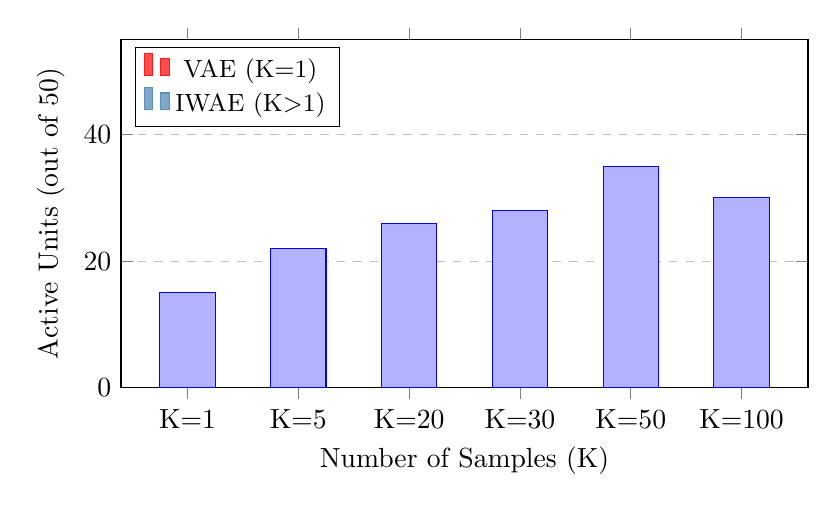
\begin{tikzpicture}
            \begin{axis}[
                ybar,
                width=0.85\textwidth,
                height=6cm,
                ylabel={Active Units (out of 50)},
                xlabel={Number of Samples (K)},
                symbolic x coords={K=1, K=5, K=20, K=30, K=50, K=100},
                xtick=data,
                ymin=0,
                ymax=55,
                nodes near coords,
                nodes near coords align={vertical},
                every node near coord/.append style={font=\scriptsize},
                bar width=20pt,
                enlarge x limits=0.12,
                legend style={at={(0.02,0.98)}, anchor=north west, font=\small},
                ymajorgrids=true,
                grid style=dashed,
                scatter,
                scatter src=explicit symbolic,
                scatter/classes={
                    vae={fill=red!70, draw=red!90},
                    iwae={fill=myBlue!70, draw=myBlue!90}
                },
            ]
            \addplot coordinates {
                (K=1, 15) [vae]
                (K=5, 22) [iwae]
                (K=20, 26) [iwae]
                (K=30, 28) [iwae]
                (K=50, 35) [iwae]
                (K=100, 30) [iwae]
            };
            \addlegendimage{fill=red!70, draw=red!90, area legend}
            \addlegendentry{VAE (K=1)}
            \addlegendimage{fill=myBlue!70, draw=myBlue!90, area legend}
            \addlegendentry{IWAE (K$>$1)}
            \end{axis}
        \end{tikzpicture}
        \caption{Number of Active Latent Dimensions (Higher is Better)}
    \end{figure}

    \textbf{Observation:} IWAE utilizes more latent dimensions, reducing ``Posterior Collapse''. Peak at K=50 (35/50 active).
\end{frame}

\subsection{K-Analysis}
\begin{frame}{Analysis: Impact of K on Training Time}
    \begin{columns}
        \column{0.55\textwidth}
        \centering
        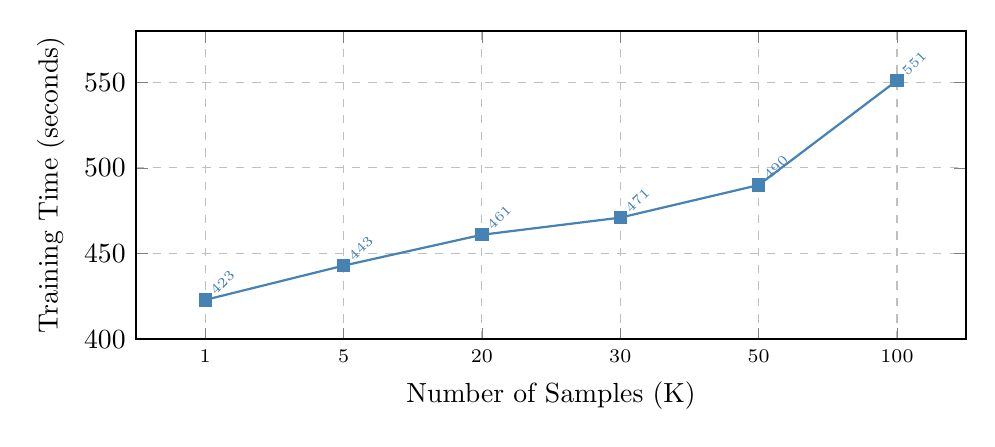
\begin{tikzpicture}
            \begin{axis}[
                width=\textwidth,
                height=5.5cm,
                xlabel={Number of Samples (K)},
                ylabel={Training Time (seconds)},
                symbolic x coords={1, 5, 20, 30, 50, 100},
                xtick=data,
                x tick label style={font=\scriptsize},
                ymin=400,
                ymax=580,
                nodes near coords,
                every node near coord/.append style={font=\tiny, rotate=45, anchor=west},
                mark=*,
                thick,
                grid=major,
                grid style=dashed,
            ]
            \addplot[color=myBlue, mark=square*, thick] coordinates {
                (1, 423)
                (5, 443)
                (20, 461)
                (30, 471)
                (50, 490)
                (100, 551)
            };
            \end{axis}
        \end{tikzpicture}

        \column{0.45\textwidth}
        \textbf{Trade-off Analysis:}
        \begin{itemize}
            \item \textbf{Compute:} Training time scales \textbf{sub-linearly} with $K$ (423s $\to$ 551s).
            \item \textbf{Log-Likelihood:} Diminishing returns as $K$ increases.
            \item \textbf{Gradient SNR:} Decreases at high $K$ (encoder neglect).
        \end{itemize}
    \end{columns}
\end{frame}

\subsection{Sample Quality}
\begin{frame}{Result 3: Sample Quality}
    \begin{columns}
        \column{0.45\textwidth}
        \centering
        \textbf{VAE (K=1)} \\
        % \includegraphics[width=0.8\textwidth]{pic/vae_samples.png}
        \rule{0.8\textwidth}{3cm} % Placeholder
        
        \column{0.45\textwidth}
        \centering
        \textbf{IWAE (K=20)} \\
        % \includegraphics[width=0.8\textwidth]{pic/iwae_samples.png}
        \rule{0.8\textwidth}{3cm} % Placeholder
    \end{columns}

    \vspace{1em}
    \centering
    \textit{IWAE samples typically show sharper strokes and fewer "averaged" blurry digits.}
\end{frame}

% =======================================================
% SECTION 4: CONCLUSION
% =======================================================
\section{Conclusion}

\begin{frame}{Trade-offs Summary}
    \begin{table}[htbp]
        \centering
        \begin{tabular}{l|c|c}
             \toprule
             \textbf{Metric} & \textbf{VAE (K=1)} & \textbf{IWAE (K=20)} \\
             \midrule
             Bound Tightness & Loose & \textbf{Tight} \\
             Latent Usage & Risk of Collapse & \textbf{Rich} \\
             Gradient Variance & High & \textbf{Low} \\
             Compute Cost & \textbf{Low} & High ($ \times K$) \\
             \bottomrule
        \end{tabular}
    \end{table}
\end{frame}

\begin{frame}
    \begin{center}
        {\Huge\textit{Thanks!}}
        
        \vspace{1cm}
        
        \textbf{Q \& A}
    \end{center}
\end{frame}

\end{document}
